% =========================================================
% Premium Beamer Visual Template Preamble
% Keep this file unchanged. Put all talk data in presentation.tex.
% =========================================================

\documentclass[aspectratio=169,11pt]{beamer}

% ---------- Packages for Beamer ----------
\usepackage[T1]{fontenc}
\usepackage[utf8]{inputenc}
\usepackage{lmodern}
\usepackage{microtype}

% ---------- Graphics and Color ----------
\usepackage{graphicx}
\usepackage{xcolor}
\usepackage{tikz}
\usetikzlibrary{
  calc,
  positioning,
  shadows.blur,
  arrows.meta,
  decorations.pathreplacing,
  shapes.geometric,
  shapes.symbols,
  fit,
  backgrounds,
  matrix
}

% ---------- Mathematics ----------
\usepackage{amsmath}
\usepackage{amssymb}
\usepackage{amsfonts}
\usepackage{mathtools}
\usepackage{bm}

% ---------- Units ----------
\usepackage{siunitx}

% ---------- Tables ----------
\usepackage{array}
\usepackage{booktabs}
\usepackage{tabularx}
\usepackage{multirow}
\usepackage{makecell}
\usepackage{colortbl}
\usepackage{adjustbox}

% ---------- Boxes and Commands ----------
\usepackage[most]{tcolorbox}
\usepackage{xparse}
\usepackage{etoolbox}
\usepackage{ragged2e}

% ---------- Code Blocks ----------
\usepackage{listings}

% ---others---
\usetikzlibrary{arrows.meta}
% ---------- Global Beamer Setup ----------
\usetheme{default}
\usefonttheme{professionalfonts}
\setbeamertemplate{navigation symbols}{}
\setbeamersize{text margin left=0.72cm,text margin right=0.72cm}
\setbeamertemplate{itemize item}{\raisebox{0.15ex}{\tiny$\blacktriangleright$}}
\setbeamertemplate{itemize subitem}{\raisebox{0.15ex}{\tiny$\bullet$}}

% ---------- Palette ----------
\definecolor{Ink}{HTML}{142033}
\definecolor{Muted}{HTML}{657084}
\definecolor{Paper}{HTML}{F6FAFD}
\definecolor{Panel}{HTML}{FFFFFF}
\definecolor{Line}{HTML}{DCE6F2}
\definecolor{Blue}{HTML}{118AB2}
\definecolor{Navy}{HTML}{073B4C}
\definecolor{Teal}{HTML}{2CB7B9}
\definecolor{Green}{HTML}{3BAA75}
\definecolor{Yellow}{HTML}{F5B82E}
\definecolor{Orange}{HTML}{F77F20}
\definecolor{Red}{HTML}{E63946}
\definecolor{Purple}{HTML}{7B61FF}
\definecolor{SoftBlue}{HTML}{EAF7FD}
\definecolor{SoftGreen}{HTML}{EDF9F2}
\definecolor{SoftYellow}{HTML}{FFF8E4}
\definecolor{SoftRed}{HTML}{FFF0F2}
\definecolor{MapBlue}{HTML}{005F99}
\definecolor{MapRed}{HTML}{B91C1C}
\definecolor{MapGreen}{HTML}{166534}
\definecolor{MapPurple}{HTML}{6D28D9}
\definecolor{MapOrange}{HTML}{A34700}
\definecolor{MapTeal}{HTML}{006D77}

\setbeamercolor{normal text}{fg=Ink,bg=Paper}
\setbeamercolor{frametitle}{fg=Ink,bg=Paper}
\setbeamercolor{structure}{fg=Blue}

% ---------- User-customizable title variables ----------
% These are redefined in presentation.tex. Preamble need not change.
\newcommand{\DeckTitle}{AI, Automation and Open Web Workflows}
\newcommand{\DeckSubtitle}{A practical visual template}
\newcommand{\PresenterName}{Presenter Name}
\newcommand{\PresenterDesignation}{Designation}
\newcommand{\PresenterAffiliation}{Affiliation}
\newcommand{\PresenterDetails}{Department / City / State}
\newcommand{\PresenterEmail}{email@example.com}
\newcommand{\EventName}{Event Name}
\newcommand{\EventDate}{Month Year}
\newcommand{\DeckTagline}{Ideas become reusable workflows when they are structured.}

% ---------- Header and footer ----------
\setbeamertemplate{headline}{%
  \leavevmode%
  \begin{beamercolorbox}[wd=\paperwidth,ht=0.36cm,dp=0.12cm,leftskip=0.72cm,rightskip=0.72cm]{normal text}%
    \scriptsize\color{Muted}\insertsection\hfill\DeckTitle%
  \end{beamercolorbox}%
  \vspace{-0.10cm}\textcolor{Line}{\rule{\paperwidth}{0.35pt}}%
}

\setbeamertemplate{footline}{%
  \leavevmode%
  \textcolor{Line}{\rule{\paperwidth}{0.35pt}}%
  \begin{beamercolorbox}[wd=\paperwidth,ht=0.34cm,dp=0.12cm,leftskip=0.72cm,rightskip=0.72cm]{normal text}%
    \scriptsize\color{Muted}\PresenterName\hfill\EventName\hfill\insertframenumber/\inserttotalframenumber%
  \end{beamercolorbox}%
}

% ---------- Frame title ----------
\setbeamertemplate{frametitle}{%
  \vspace{0.18cm}%
  \begin{beamercolorbox}[wd=\textwidth,ht=0.62cm,dp=0.08cm]{frametitle}%
    \usebeamerfont{frametitle}\bfseries\Large\insertframetitle%
  \end{beamercolorbox}%
  \vspace{-0.12cm}%
}

% ---------- Text helpers ----------
\newcommand{\SmallNote}[1]{\vfill{\scriptsize\color{Muted}#1}}

\newtcolorbox{PremiumCard}[1][]{%
  enhanced,
  colback=Panel,
  colframe=Line,
  boxrule=0.5pt,
  arc=3mm,
  left=2.8mm,right=2.8mm,top=2.2mm,bottom=2.2mm,
  drop shadow={shadow xshift=0.7mm,shadow yshift=-0.7mm,opacity=0.13},
  #1
}

\newcommand{\Pill}[2][Blue]{%
  \tikz[baseline=(X.base)]\node[rounded corners=7pt,inner xsep=7pt,inner ysep=2pt,fill=#1!10,draw=#1!25,text=#1,font=\scriptsize\bfseries](X){#2};%
}



\usepackage{listings}

\lstdefinestyle{PremiumCode}{
  basicstyle=\ttfamily\scriptsize,
  columns=fullflexible,
  breaklines=true,
  breakatwhitespace=false,
  showstringspaces=false,
  keepspaces=true,
  frame=none,
  backgroundcolor=\color{white},
  keywordstyle=\color{Blue}\bfseries,
  commentstyle=\color{Muted},
  stringstyle=\color{Teal}
}

\newtcblisting{PremiumCodeBox}[1][]{%
  enhanced,
  listing only,
  listing engine=listings,
  colback=Panel,
  colframe=Line,
  boxrule=0.5pt,
  arc=3mm,
  left=2.2mm,right=2.2mm,top=1.8mm,bottom=1.8mm,
  drop shadow={shadow xshift=0.7mm,shadow yshift=-0.7mm,opacity=0.13},
  listing options={style=PremiumCode,#1}
}



% ---------- Title-slide right image card ----------
\newcommand{\TitleImageCard}[1]{%
\begin{minipage}{0.33\textwidth}
\centering
\begin{tikzpicture}

  % fixed dimensions
  \def\cardw{5.50cm}
  \def\cardh{3.80cm}
  \def\radius{16pt}

  % soft shadow
  \fill[
    black,
    opacity=0.22,
    rounded corners=\radius
  ]
  (0.12,-0.12) rectangle (\cardw,-\cardh);

  % rounded clipping region
  \begin{scope}
    \clip[
      rounded corners=\radius
    ]
    (0,0) rectangle (\cardw,-\cardh);

    % image forced into fixed size
    \node[
      anchor=north west,
      inner sep=0pt,
      outer sep=0pt
    ]
    at (0,0)
    {
      \includegraphics[
        width=\cardw,
        height=\cardh
      ]{#1}
    };
  \end{scope}

\end{tikzpicture}
\end{minipage}
}


% ---------- Premium title slide ----------
\newcommand{\PremiumTitleSlide}{%
\begin{frame}[plain]
\begin{tikzpicture}[remember picture,overlay]
  \fill[Paper] (current page.south west) rectangle (current page.north east);
  \fill[Blue!8] (current page.south west) rectangle ([xshift=\paperwidth]current page.north west);

  \fill[Navy] 
  ([xshift=0.50\paperwidth]current page.south west)
  .. controls 
  ([xshift=0.90\paperwidth,yshift=0.28\paperheight]current page.south west)
  and 
  ([xshift=0.20\paperwidth,yshift=0.50\paperheight]current page.south west)
  ..
  ([xshift=0.90\paperwidth]current page.north west)
  -- (current page.north east)
  -- (current page.south east)
  -- cycle;

  \foreach \x/\y/\c in {0.76/0.81/Yellow,0.80/0.73/Teal,0.86/0.86/Red,0.92/0.62/Purple}
  {
    \fill[\c] ([xshift=\x\paperwidth,yshift=\y\paperheight]current page.south west) circle (1.4pt);
  }
\end{tikzpicture}

\vspace{0.55cm}

\begin{minipage}{0.58\textwidth}
\raggedright
{\bfseries\fontsize{24}{27}\selectfont\color{Ink}\DeckTitle\par}
\vspace{0.14cm}

{\large\color{Blue}\bfseries\DeckSubtitle\par}
\vspace{0.34cm}

{\bfseries\Large\color{Ink}\PresenterName\par}
\vspace{0.06cm}

{\color{Muted}\PresenterDesignation\par}
\vspace{0.05cm}

{\color{Muted}\PresenterAffiliation\par}
\vspace{0.05cm}

{\scriptsize\color{Muted}\PresenterDetails\par}
\vspace{0.14cm}

{\scriptsize\color{Muted}\PresenterEmail\par}
\vspace{0.42cm}

\Pill[Blue]{\EventName}\hspace{0.12cm}\Pill[Yellow]{\EventDate}

\vspace{0.42cm}
{\scriptsize\color{Muted}\DeckTagline}
\end{minipage}
\hfill
\TitleImageCard{\TitleRightImage}

\end{frame}
}






% ---------- Diagram color helpers ----------
\newcount\DeckDiagramCount
\newcommand{\DeckDiagramColor}[1]{%
  \ifcase#1 Navy\or MapBlue\or MapRed\or MapGreen\or MapPurple\or MapOrange\or MapTeal\else Navy\fi%
}

% ---------- Wheel diagram commands ----------
% Simple workflow:
% \WheelDiagram{WORKFLOW}{AI, Agents, Codex, Automation}
% Up to six comma-separated labels are used.
\NewDocumentCommand{\WheelDiagram}{m m}{%
\DeckDiagramCount=0
\foreach \lbl in {#2}{\global\advance\DeckDiagramCount by 1}%
\ifnum\DeckDiagramCount<1 \DeckDiagramCount=1 \fi
\ifnum\DeckDiagramCount>6 \DeckDiagramCount=6 \fi
\begin{tikzpicture}[scale=0.90, every node/.style={font=\scriptsize\bfseries}]
  \def\WheelOuter{2.15}
  \def\WheelInner{0.72}
  \foreach \lbl [count=\i from 1] in {#2}{%
    \ifnum\i>\DeckDiagramCount\relax\else
      \pgfmathsetmacro{\a}{90-(\i-1)*360/\the\DeckDiagramCount}
      \pgfmathsetmacro{\b}{90-\i*360/\the\DeckDiagramCount}
      \pgfmathsetmacro{\m}{(\a+\b)/2}
      \path[fill=\DeckDiagramColor{\i},draw=white,line width=1.8pt]
        (\a:\WheelInner) -- (\a:\WheelOuter)
        arc[start angle=\a,end angle=\b,radius=\WheelOuter]
        -- (\b:\WheelInner)
        arc[start angle=\b,end angle=\a,radius=\WheelInner] -- cycle;
      \node[text=white,align=center,font=\scriptsize\bfseries] at (\m:1.46) {\lbl};
    \fi
  }%
  \fill[white,blur shadow={shadow blur steps=6,shadow opacity=0.16}] (0,0) circle (0.82);
  \draw[Line,line width=1pt] (0,0) circle (0.82);
  \node[align=center,text=Ink,font=\scriptsize\bfseries] at (0,0) {#1};
\end{tikzpicture}%
}

% Backward-compatible wheel command for older slides.
\newcommand{\Wheel}[8]{%
\begin{tikzpicture}[scale=0.90, every node/.style={font=\scriptsize\bfseries}]
  \def\R{2.15}
  \def\r{0.72}
  \pgfmathtruncatemacro{\N}{#2}
  \ifnum\N<1\pgfmathtruncatemacro{\N}{1}\fi
  \ifnum\N>6\pgfmathtruncatemacro{\N}{6}\fi
  \foreach \i/\lbl/\col in {1/{#3}/MapBlue,2/{#4}/MapRed,3/{#5}/MapGreen,4/{#6}/MapPurple,5/{#7}/MapOrange,6/{#8}/MapTeal}{%
    \ifnum\i>\N\relax\else
      \pgfmathsetmacro{\a}{90-(\i-1)*360/\N}
      \pgfmathsetmacro{\b}{90-\i*360/\N}
      \pgfmathsetmacro{\m}{(\a+\b)/2}
      \path[fill=\col,draw=white,line width=1.8pt]
        (\a:\r) -- (\a:\R) arc[start angle=\a,end angle=\b,radius=\R] -- (\b:\r) arc[start angle=\b,end angle=\a,radius=\r] -- cycle;
      \node[text=white,align=center,font=\scriptsize\bfseries] at (\m:1.46) {\lbl};
    \fi
  }%
  \fill[white,blur shadow={shadow blur steps=6,shadow opacity=0.16}] (0,0) circle (0.82);
  \draw[Line,line width=1pt] (0,0) circle (0.82);
  \node[align=center,text=Ink,font=\scriptsize\bfseries] at (0,0) {#1};
\end{tikzpicture}%
}





% ---------- Flexible category map command ----------
% Simple workflow:
% \CategoryMap{Topics}{AI, Automation, Workflow}
% Up to six comma-separated labels are used.
\NewDocumentCommand{\CategoryMap}{m m}{%
\DeckDiagramCount=0
\foreach \lbl in {#2}{\global\advance\DeckDiagramCount by 1}%
\ifnum\DeckDiagramCount<1 \DeckDiagramCount=1 \fi
\ifnum\DeckDiagramCount>6 \DeckDiagramCount=6 \fi
\begin{tikzpicture}[every node/.style={font=\scriptsize\bfseries}]

  % Root title
  \def\RootTitle{#1}

  % Root node
  \node[
    rounded corners=12pt,
    fill=Navy,
    text=white,
    inner xsep=12pt,
    inner ysep=7pt
  ] (root) at (0,0) {\RootTitle};

  % Draw branches
  \foreach \lbl [count=\i from 1] in {#2}{%
    \ifnum\i>\DeckDiagramCount\relax\else
      \pgfmathsetmacro{\a}{90 - (360/\the\DeckDiagramCount)*(\i-1)}
      \pgfmathsetmacro{\x}{2.60*cos(\a)}
      \pgfmathsetmacro{\y}{2.60*sin(\a)}
      \node[
        rounded corners=8pt,
        fill=\DeckDiagramColor{\i},
        draw=white,
        line width=0.8pt,
        text=white,
        inner xsep=8pt,
        inner ysep=4pt,
        align=center
      ] (n\i) at (\x,\y) {\lbl};
      \draw[-{Latex[length=2.2mm]},line width=0.8pt,draw=\DeckDiagramColor{\i}] (root) -- (n\i);
    \fi
  }%

\end{tikzpicture}
}





% ---------- Premium image placement command ----------
% Usage: \PremiumImage[0.78\textwidth]{img/file.jpeg}{Caption text}
\NewDocumentCommand{\PremiumImage}{O{0.82\textwidth} m m}{%
\begin{PremiumCard}[left=2mm,right=2mm,top=2mm,bottom=1.4mm]
  \centering
  \includegraphics[width=#1,keepaspectratio]{#2}\par
  \vspace{0.07cm}
  {\scriptsize\color{Muted}#3}
\end{PremiumCard}%
}

% ---------- Slide layout helpers ----------
\newcommand{\TwoCol}[4]{%
\begin{columns}[T,onlytextwidth]
\begin{column}{#1}\raggedright #2\end{column}
\begin{column}{#3}\raggedright #4\end{column}
\end{columns}%
}

% Default two-column slide layout. Use \TwoCol only when custom widths are needed.
\newcommand{\TwoColumns}[2]{%
\TwoCol{0.48\textwidth}{#1}{0.48\textwidth}{#2}%
}

\newcommand{\CommandCard}[2]{%
\begin{PremiumCard}
{\bfseries\color{Blue}#1}\par\vspace{0.08cm}
{\scriptsize\ttfamily\color{Ink}#2}
\end{PremiumCard}%
}

\NewDocumentCommand{\DiagramCard}{O{0.90\linewidth} m}{%
\begin{PremiumCard}
\centering
\resizebox{#1}{!}{#2}
\end{PremiumCard}%
}

\NewDocumentCommand{\FullSlideMap}{m m}{%
\vspace{-0.10cm}
\begin{center}
\resizebox{!}{0.66\textheight}{\CategoryMap{#1}{#2}}
\end{center}%
}

\NewDocumentCommand{\FullSlideWheel}{m m}{%
\vspace{-0.06cm}
\begin{center}
\resizebox{!}{0.64\textheight}{\WheelDiagram{#1}{#2}}
\end{center}%
}

% Short user-facing aliases for simple slide writing.
\NewDocumentCommand{\MapSlide}{m m}{\FullSlideMap{#1}{#2}}
\NewDocumentCommand{\WheelSlide}{m m}{\FullSlideWheel{#1}{#2}}
\NewDocumentCommand{\MapOnly}{O{0.90\linewidth} m m}{%
\resizebox{#1}{!}{\CategoryMap{#2}{#3}}%
}
\NewDocumentCommand{\WheelOnly}{O{0.90\linewidth} m m}{%
\resizebox{#1}{!}{\WheelDiagram{#2}{#3}}%
}
\NewDocumentCommand{\MapCard}{O{0.90\linewidth} m m}{%
\begin{PremiumCard}
\centering
\MapOnly[#1]{#2}{#3}
\end{PremiumCard}%
}
\NewDocumentCommand{\WheelCard}{O{0.90\linewidth} m m}{%
\begin{PremiumCard}
\centering
\WheelOnly[#1]{#2}{#3}
\end{PremiumCard}%
}
\NewDocumentCommand{\Split}{+m +m}{\TwoColumns{#1}{#2}}
\NewDocumentCommand{\Cols}{m +m m +m}{\TwoCol{#1}{#2}{#3}{#4}}
\NewDocumentCommand{\ImageCard}{O{0.82\textwidth} m m}{\PremiumImage[#1]{#2}{#3}}
\newenvironment{Card}{\begin{PremiumCard}}{\end{PremiumCard}}

% ---------- Part breaker slide ----------
% Usage: \PartSlide{1}{AI: Prompting, agents and Codex}
\NewDocumentCommand{\PartCanvas}{m m}{%
\begin{tikzpicture}[x=\paperwidth,y=\paperheight]
  \fill[Ink!88!black] (0,0) rectangle (1,1);
  \fill[Blue] (0,0.78) rectangle (1,1);
  \node[
    text=white,
    font=\bfseries\fontsize{38}{42}\selectfont
  ] at (0.12,0.89) {#1};
  \node[
    anchor=west,
    align=left,
    text=white,
    text width=0.68\paperwidth,
    font=\bfseries\fontsize{30}{35}\selectfont
  ] at (0.25,0.50) {#2};
  \draw[Yellow,line width=1.6pt] (0.25,0.33) -- (0.78,0.33);
\end{tikzpicture}%
}

\NewDocumentCommand{\PartPreview}{m m}{%
\begin{PremiumCard}
\centering
\resizebox{0.95\linewidth}{!}{\PartCanvas{#1}{#2}}
\end{PremiumCard}%
}

\NewDocumentCommand{\PartSlide}{m m}{%
\begin{frame}[plain]
\begin{tikzpicture}[remember picture,overlay]
  \fill[Ink!88!black] (current page.south west) rectangle (current page.north east);
  \fill[Blue] ([yshift=0.78\paperheight]current page.south west) rectangle (current page.north east);
  \node[
    text=white,
    font=\bfseries\fontsize{38}{42}\selectfont
  ] at ([xshift=0.12\paperwidth,yshift=0.89\paperheight]current page.south west) {#1};
  \node[
    anchor=west,
    align=left,
    text=white,
    text width=0.68\paperwidth,
    font=\bfseries\fontsize{30}{35}\selectfont
  ] at ([xshift=0.25\paperwidth,yshift=0.50\paperheight]current page.south west) {#2};
  \draw[Yellow,line width=1.6pt]
    ([xshift=0.25\paperwidth,yshift=0.33\paperheight]current page.south west)
    --
    ([xshift=0.78\paperwidth,yshift=0.33\paperheight]current page.south west);
\end{tikzpicture}
\end{frame}%
}


% =========================================================
% Simple workflow:
% 1. Edit the title data below.
% 2. Add slides after \PremiumTitleSlide.
% 3. Keep reusable layout, image, wheel, and map code in preamble.tex.
% =========================================================

% ---------- Title-page data ----------
\renewcommand{\DeckTitle}{AI, Automation and Open Web Workflows}
\renewcommand{\DeckSubtitle}{Converting scattered knowledge into reusable workflows, diagrams, and publishable web material.}
\renewcommand{\PresenterName}{Rajesh Kumar}
\renewcommand{\PresenterDesignation}{Assistant Professor, Department of Physics}
\renewcommand{\PresenterAffiliation}{Sido Kanhu Murmu University, Dumka, Jharkhand}
\renewcommand{\PresenterDetails}{M.Sc. Physics, IIT Kanpur}
\renewcommand{\PresenterEmail}{kr.rajesh.phy@gmail.com}
\renewcommand{\EventName}{UGC MMTTC Refresher Course}
\renewcommand{\EventDate}{June 2026}
\renewcommand{\DeckTagline}{Refresher Course in Information Technology}
\newcommand{\TitleRightImage}{img/title-image.png}

\begin{document}

\PremiumTitleSlide




\section{OVERVIEW}
\begin{frame}{Topics We Will Discuss}
\MapSlide{Topics}{AI, Automation, Workflow}
\end{frame}

\PartSlide{1}{Artificial Intelligence}

\section{AI}

\begin{frame}{What comes to mind when you think of AI?}
\Split{
  \PremiumImage[0.25\linewidth]{img/gemini.jpeg}{}
  \PremiumImage[0.20\linewidth]{img/chatgpt.png}{}
  \PremiumImage[0.20\linewidth]{img/claude.png}{}}{
    \PremiumImage[0.25\linewidth]{img/perplexity.jpeg}{}
    \PremiumImage[0.25\linewidth]{img/llama.png}{}
    \PremiumImage[0.25\linewidth]{img/grok.png}{}
  }
\end{frame}



\begin{frame}{AI USE Framework}
\Split{
\begin{itemize}\scriptsize
  \item \textbf{Organize}: Collect scattered notes, PDFs, screenshots, and ideas into clear folders, chapters, slides, or web posts.
  \item \textbf{Automate}: Make repeated work one-command, such as downloading PDFs, merging files, fetching weather, or compiling LaTeX.
  \item \textbf{Visualize}: Turn ideas into diagrams, charts, Beamer slides, TikZ figures, and clean academic templates.
  \item \textbf{Publish}: Convert organized material into PDFs, websites, GitHub pages, blogs, and reusable teaching resources.
\end{itemize}
}{
\PremiumImage[\linewidth]{img/4-work.png}{}
}
\end{frame}


\begin{frame}{Repetitive Tasks; Connecting Tools}
\Split{
\begin{PremiumCard}
{\bfseries\color{Blue}AI can generate code}\par
\vspace{0.12cm}
\begin{itemize}\scriptsize
  \item AI can write code in many programming languages.
  \item Latex, Python, HTML, JavaScript, and more.
  \item AI can also explain code and debug errors.
\end{itemize}
\PremiumImage[0.4\linewidth]{img/linux.jpeg}{}
\end{PremiumCard}
}{\PremiumImage[0.2\linewidth]{img/latex.png}{}
\PremiumImage[0.2\linewidth]{img/python.jpeg}{}
\PremiumImage[0.3\linewidth]{img/html.jpeg}{}
\PremiumImage[0.2\linewidth]{img/jekyll.png}{}
}
\end{frame}


\begin{frame}{}
  \centering
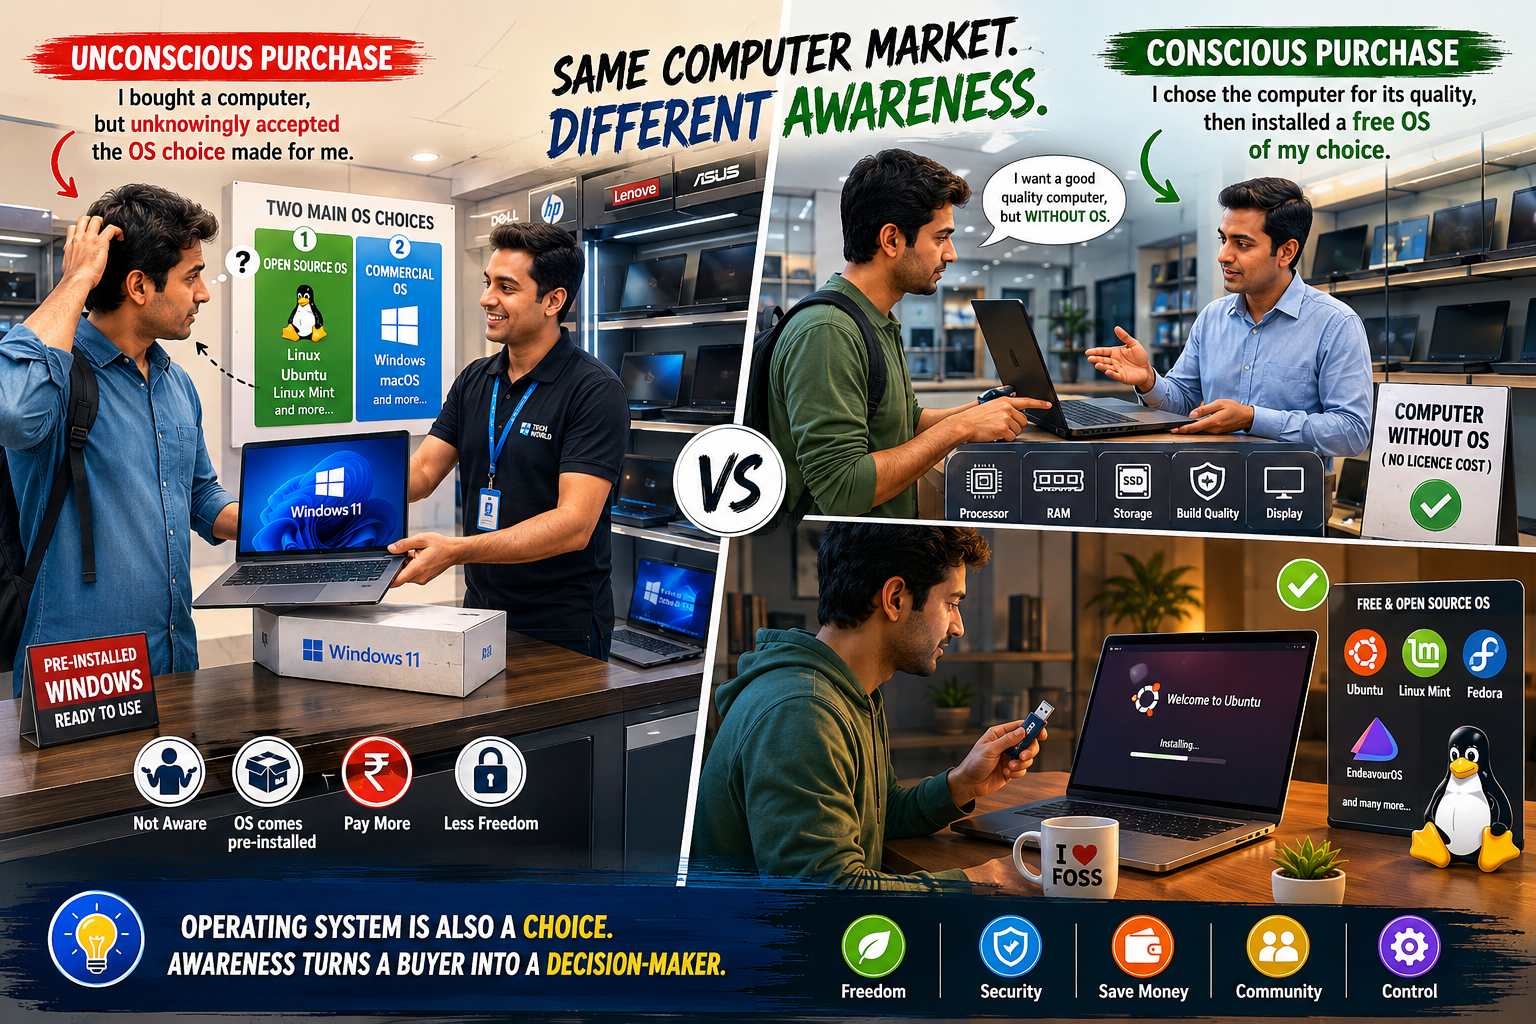
\includegraphics[width=0.9\linewidth]{img/OS-Choice.png}
\end{frame}

\begin{frame}{}
  \centering

\includegraphics[width=0.9\linewidth]{img/AI-Bridge.png}
\end{frame}



\begin{frame}{Coding For Weather Forecast Report Download}
\Split{
\PremiumImage[\linewidth]{img/weather.png}{}
}{
\PremiumImage[\linewidth]{img/code.png}{}
}
\end{frame}




\begin{frame}{Workflow Easily Achieved Using Coding Agents}
  \Split{
  \begin{PremiumCard}
  {\WheelCard{USE}{Organize, Automate,Visualize, Publish}}
  \end{PremiumCard}
  }{
    \PremiumImage[0.3\linewidth]
    {img/codex.jpeg}
    {Codex}
    \PremiumImage[0.3\linewidth]
    {img/claude.png}
    {Claude}
  }
\end{frame}



\PartSlide{2}{Automation}

\section{Automation}

\begin{frame}{Task Types for Automation}
\Split{\PremiumImage[\linewidth]{img/task.png}{}
}
{
  \begin{PremiumCard}
{\bfseries\color{Blue}1. Downloading Monthly Journals}\par
\end{PremiumCard}

\begin{PremiumCard}
{\bfseries\color{Green}2. Opening News}\par
\end{PremiumCard}

\begin{PremiumCard}
{\bfseries\color{Blue}3. Image and Video Files Processing}\par
\end{PremiumCard}

\begin{PremiumCard}
{\bfseries\color{Orange}4. Accessing Files in One Click}\par
\end{PremiumCard}
}
\end{frame}


\begin{frame}{}
  \centering
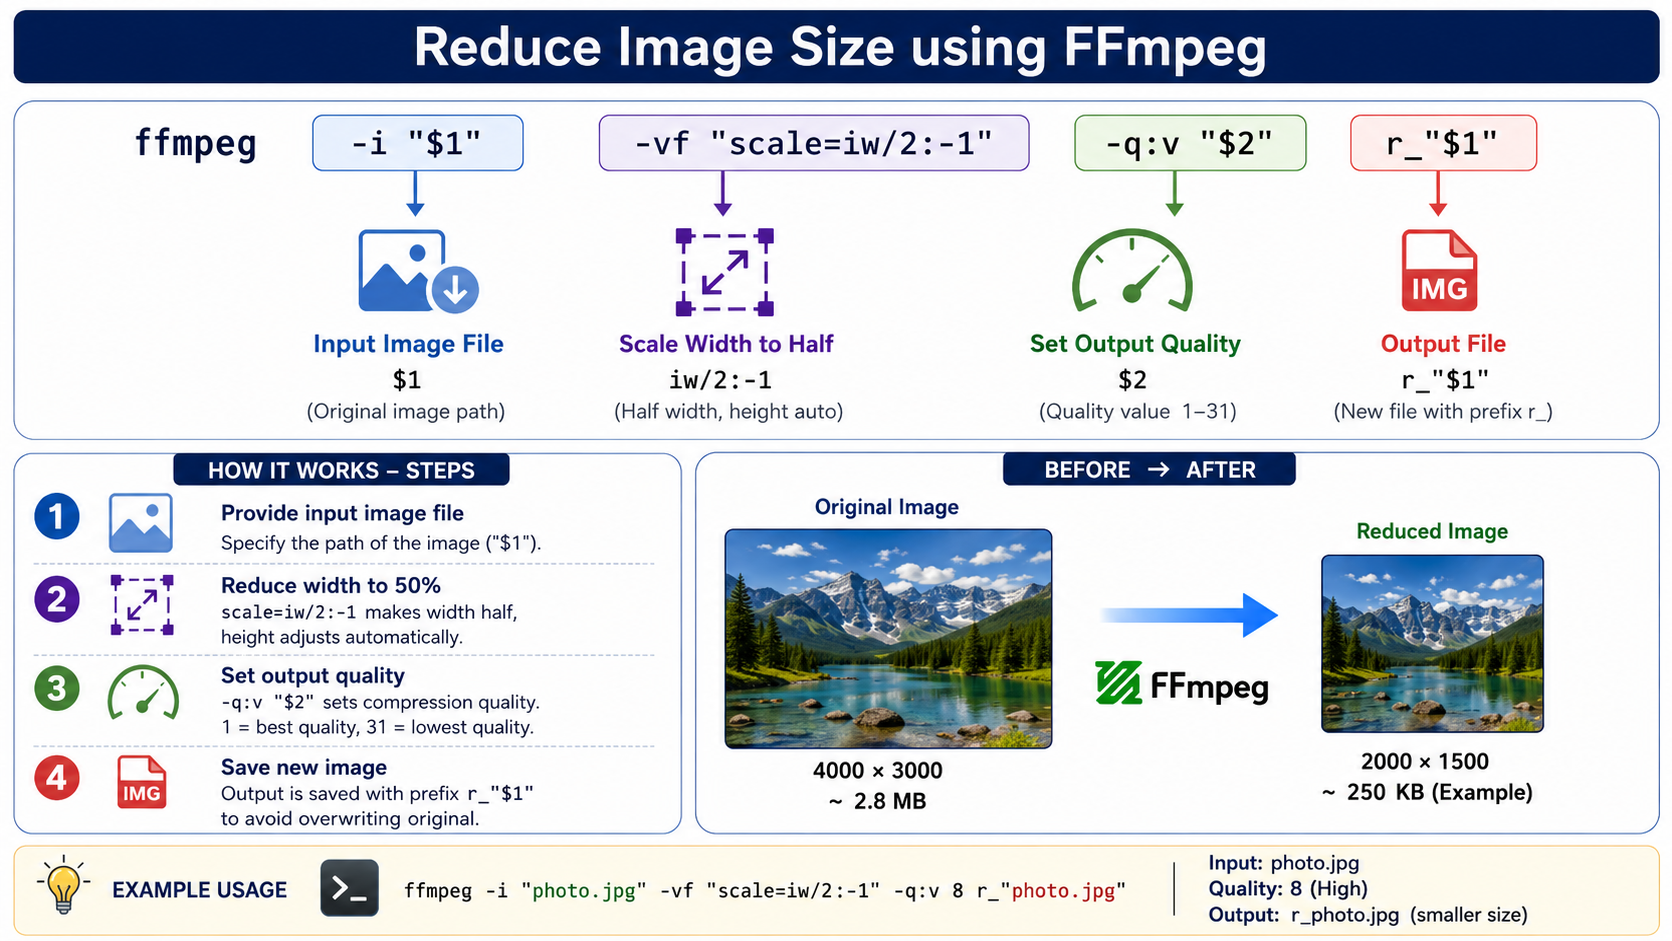
\includegraphics[width=0.9\linewidth]{img/ffmpeg.png}
\end{frame}





\begin{frame}{Automating Journal Download}
\Split{
  \PremiumImage[\linewidth]{img/journal.png}{}
}{
  \begin{PremiumCard}
{\bfseries\color{Blue}Journal issue to book-form PDF}\par
\vspace{0.12cm}
\begin{enumerate}\scriptsize
  \item Enter volume and issue number.
  \item Check whether the PDF already exists.
  \item Fetch the page numbers from the website.
  \item Extract article page ranges and titles.
  \item Download the cover page of the issue.
  \item Build direct PDF links for all articles.
  \item Download all article PDFs.
  \item Create a table-of-contents.
  \item Merge cover, TOC, and articles in one PDF.
  \item Remove temp files and open the final PDF.
\end{enumerate}
\end{PremiumCard}
}
\end{frame}



\section{Website Workflows}

\PartSlide{3}{Web Workflows}

\section{AUTOMATING WEB WORKFLOWS}

\begin{frame}{What Is a Web Page?}
\TwoCol{0.48\textwidth}{
\begin{PremiumCard}
{\bfseries\color{Blue}Web page = HTML structure}\par
\vspace{0.12cm}
\begin{itemize}\scriptsize
  \item A web page is built from HTML.
  \item HTML gives the page its basic structure.
  \item Headings, paragraphs, links, images, and sections are HTML elements.
  \item What we see in the browser has a code background.
\end{itemize}
\end{PremiumCard}
}{0.48\textwidth}{
\PremiumImage[0.95\linewidth]{img/web-page-html.png}{}
}
\end{frame}

\begin{frame}{Styles, Functions and Fonts}
\TwoCol{0.48\textwidth}{
\begin{PremiumCard}
{\bfseries\color{Blue}CSS and JavaScript add life}\par
\vspace{0.12cm}
\begin{itemize}\scriptsize
  \item CSS controls colors, spacing, fonts, cards, and layout.
  \item JavaScript controls interaction and dynamic behavior.
  \item Bootstrap gives ready-made design components.
  \item Together they turn plain HTML into a modern page.
\end{itemize}
\end{PremiumCard}
}{0.48\textwidth}{
\PremiumImage[0.95\linewidth]{img/css-js-style-function.png}{}
}
\end{frame}

\begin{frame}{Static vs Dynamic Websites}
\TwoCol{0.48\textwidth}{
\begin{PremiumCard}
{\bfseries\color{Blue}Two kinds of websites}\par
\vspace{0.12cm}
\begin{itemize}\scriptsize
  \item Static websites are pre-built pages served directly.
  \item Dynamic websites generate pages using databases and server logic.
  \item Static sites are faster, simpler, and easier to host.
  \item Dynamic sites are useful when content changes for every user.
\end{itemize}
\end{PremiumCard}
}{0.48\textwidth}{
\PremiumImage[0.95\linewidth]{img/static-vs-dynamic.png}{}
}
\end{frame}

\begin{frame}{Jekyll as a Workflow Solver}
\TwoCol{0.48\textwidth}{
\begin{PremiumCard}
{\bfseries\color{Blue}Write once, organize automatically}\par
\vspace{0.12cm}
\begin{itemize}\scriptsize
  \item Jekyll converts Markdown into web pages.
  \item Posts, pages, categories, tags, and links become organized.
  \item GitHub Pages can publish the site directly.
  \item This makes scattered notes reusable and publishable.
\end{itemize}
\end{PremiumCard}
}{0.48\textwidth}{
\PremiumImage[0.95\linewidth]{img/jekyll-workflow.png}{}
}
\end{frame}






\PartSlide{4}{Publishing with Jekyll and GitHub Pages}

\section{JEKYLL AND GITHUB PAGES}

\begin{frame}{Why Jekyll?}
\TwoCol{0.48\textwidth}{
\begin{PremiumCard}
{\bfseries\color{Blue}Jekyll solves the publishing problem}\par
\vspace{0.12cm}
\begin{itemize}\scriptsize
  \item Write content once in Markdown.
  \item Jekyll converts it into a static website.
  \item Posts, pages, categories, and layouts become organized automatically.
  \item Other popular static-site tools include Hugo, MkDocs, Astro, Eleventy, and Docusaurus.
\end{itemize}
\end{PremiumCard}

}{0.48\textwidth}{
\begin{PremiumCard}
\MapCard{Static}{Jekyll, Hugo, MkDocs, Astro, Eleventy, Docusaurus}
\end{PremiumCard}
}
\end{frame}




\begin{frame}{GitHub as a Free Repository}
\TwoCol{0.48\textwidth}{
\begin{PremiumCard}
{\bfseries\color{Blue}GitHub stores your project files}\par
\vspace{0.12cm}
\begin{itemize}\scriptsize
  \item A repository is a project folder stored online.
  \item It can keep code, notes, images, PDFs, and website files.
  \item GitHub supports version history and collaboration.
  \item Public repositories can be used freely for open academic material.
\end{itemize}
\end{PremiumCard}
}{0.48\textwidth}{
\PremiumImage[0.95\linewidth]{img/github-free-repository.png}{}
}
\end{frame}

\begin{frame}{GitHub Pages: Free Website Hosting}
\TwoCol{0.48\textwidth}{
\begin{PremiumCard}
{\bfseries\color{Blue}From repository to website}\par
\vspace{0.12cm}
\begin{itemize}\scriptsize
  \item GitHub Pages publishes static websites from a repository.
  \item It has built-in support for Jekyll.
  \item A user website can appear as \texttt{username.github.io}.
  \item This is useful for teaching notes, academic pages, blogs, and documentation.
\end{itemize}
\end{PremiumCard}
}{0.48\textwidth}{
\PremiumImage[0.95\linewidth]{img/github-pages-free-website.png}{}
}
\end{frame}

\begin{frame}{My Website}
\begin{PremiumCard}
\centering
{\bfseries\color{Blue}Type this URL in your browser}\par
\vspace{0.35cm}

{\fontsize{34}{40}\selectfont\bfseries\color{Ink}
rajeshphy.github.io
\par}

\vspace{0.35cm}
\PremiumImage[0.4\linewidth]{img/rajeshphy-website-url.png}{}
\end{PremiumCard}
\end{frame}







\begin{frame}[plain]

\begin{tikzpicture}[remember picture,overlay]
  \fill[Paper] (current page.south west) rectangle (current page.north east);

  % soft background circles
  \fill[Blue!10] 
    ([xshift=-1.8cm,yshift=1.2cm]current page.south west) circle (3.2cm);
  \fill[Teal!10] 
    ([xshift=1.4cm,yshift=-0.9cm]current page.north east) circle (3.5cm);
  \fill[Yellow!18] 
    ([xshift=0.6cm,yshift=0.4cm]current page.center) circle (1.6cm);
\end{tikzpicture}

\vspace{1.05cm}

\begin{center}

\begin{PremiumCard}
\centering

{\fontsize{42}{48}\selectfont\bfseries\color{Ink}
Thank You
\par}

\vspace{0.28cm}

{\Large\bfseries\color{Blue}
Questions and Discussion
\par}

\vspace{0.45cm}

{\small\color{Muted}
AI, Automation and Open Web Workflows
\par}

\vspace{0.35cm}

{\bfseries\color{Ink}
Rajesh Kumar
\par}

{\scriptsize\color{Muted}
Assistant Professor, Department of Physics\\
Sido Kanhu Murmu University, Dumka, Jharkhand
\par}

\vspace{0.35cm}

{\fontsize{20}{24}\selectfont\bfseries\color{Blue}
rajeshphy.github.io
\par}

\vspace{0.15cm}

{\scriptsize\color{Muted}
kr.rajesh.phy@gmail.com
\par}

\end{PremiumCard}

\end{center}

\end{frame}


\end{document}
